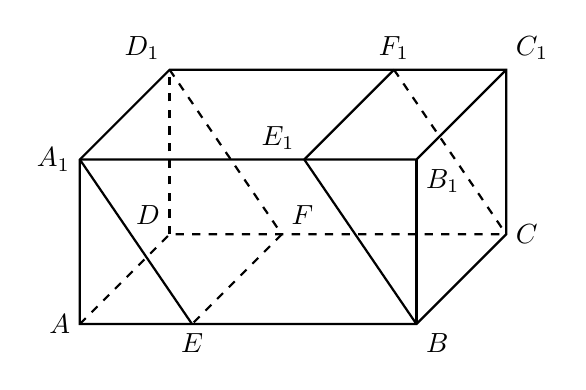
\begin{tikzpicture}[>=stealth, scale=0.95]
  % 顶点坐标
  \coordinate (A) at (0, 0);
  \coordinate (B) at (4.5, 0);
  \coordinate (C) at (5.7, 1.2);
  \coordinate (D) at (1.2, 1.2);

  \coordinate (A1) at (0, 2.2);
  \coordinate (B1) at (4.5, 2.2);
  \coordinate (C1) at (5.7, 3.4);
  \coordinate (D1) at (1.2, 3.4);

  % 截面分点 E, F, E1, F1 (比例 1:4:1, 即 1/6 与 5/6 处)
  % AB 长 4.5, E 在 1/3 (1.5) 处
  \coordinate (E) at (1.5, 0);
  \coordinate (F) at (2.7, 1.2);
  \coordinate (E1) at (3.0, 2.2);
  \coordinate (F1) at (4.2, 3.4);

  % 可见外框与实线
  \draw[thick] (A) -- (B) -- (C) -- (C1) -- (D1) -- (A1) -- cycle;
  \draw[thick] (A1) -- (B1) -- (C1);
  \draw[thick] (B) -- (B1);

  % 截面可见线
  \draw[thick] (A1) -- (E);
  \draw[thick] (E1) -- (B);
  \draw[thick] (E1) -- (F1);

  % 虚线（内部与被遮挡线）
  \draw[dashed, thick] (A) -- (D) -- (C);
  \draw[dashed, thick] (D) -- (D1);
  \draw[dashed, thick] (D1) -- (F) -- (E);
  \draw[dashed, thick] (F1) -- (C);

  % 节点标注
  \node[left] at (A) {$A$};
  \node[below right] at (B) {$B$};
  \node[right] at (C) {$C$};
  \node[above left] at (D) {$D$};

  \node[left] at (A1) {$A_1$};
  \node[below right] at (B1) {$B_1$};
  \node[above right] at (C1) {$C_1$};
  \node[above left] at (D1) {$D_1$};

  \node[below] at (E) {$E$};
  \node[above right] at (F) {$F$};
  \node[above left] at (E1) {$E_1$};
  \node[above] at (F1) {$F_1$};
\end{tikzpicture}
